\documentclass[10pt,aspectratio=43,mathserif,table]{beamer} 
%  设置为 Beamer 文档类型,设置字体为 10pt,长宽比为16:9,数学字体为 serif 风格
\batchmode
\usepackage{graphicx}
\usepackage{subfigure}
\usepackage{fontspec}
\usepackage{multicol}

% \setmainfont{Harding Text Web Regular Regular.ttf}
\usepackage{diagbox} % 表头斜线分区
\usepackage{unicode-math}
\usefonttheme{serif}

\usetheme{Berlin} %主题
\setbeamertemplate{page number in head/foot}[pagenumber]
%\usecolortheme{sustech} %主题颜色

\usepackage[ruled,linesnumbered]{algorithm2e}

\usepackage{fancybox}
\usepackage{xcolor}
\usepackage{listings}

\usepackage{booktabs}
\usepackage{colortbl}

\newcommand{\Console}{Console}
\lstset{ %
	backgroundcolor=\color{white},   % choose the background color
	basicstyle=\footnotesize\rmfamily,     % size of fonts used for the code
	columns=fullflexible,
	breaklines=true,                 % automatic line breaking only at whitespace
	captionpos=b,                    % sets the caption-position to bottom
	tabsize=4,
	commentstyle=\color{mygreen},    % comment style
	escapeinside={\%*}{*)},          % if you want to add LaTeX within your code
	keywordstyle=\color{blue},       % keyword style
	stringstyle=\color{mymauve}\ttfamily,     % string literal style
	numbers=left, 
	%	frame=single,
	rulesepcolor=\color{red!20!green!20!blue!20},
	% identifierstyle=\color{red},
	language=c
}


\definecolor{mygreen}{rgb}{0,0.6,0}
\definecolor{mymauve}{rgb}{0.58,0,0.82}
\definecolor{mygray}{gray}{.9}
\definecolor{mypink}{rgb}{.99,.91,.95}
\definecolor{mycyan}{cmyk}{.3,0,0,0}

%题目,作者,学校,日期
\title{H.Haken - Synergetics, An Introduction \newline 1. Goal - 2. Probability}
%\subtitle{\fontsize{9pt}{14pt}\textbf{跨临界分岔}}
\author{Speaker: Yichen Lu (Systems Science)\quad \newline  \newline \quad }
\institute{School of Mathematical Science}
\date{\today}
\newcommand{\concept}{Paper Reading}

%学校Logo
%\pgfdeclareimage[height=0.5cm]{sustech-logo}{sustech-logo.pdf}
%\logo{\pgfuseimage{sustech-logo}\hspace*{0.3cm}}

\AtBeginSection[]
{
	\begin{frame}<beamer>
	\frametitle{\textbf{Contents}}
	\tableofcontents[currentsection]
\end{frame}
}
% \beamerdefaultoverlayspecification{<+->}
% -----------------------------------------------------------------------------
\begin{document}
% -----------------------------------------------------------------------------

\frame{\titlepage}
\section{Goal}
\subsection{Order and Disorder: Some Typical Phenomena}
\begin{frame}
    \begin{figure}
        \centering
        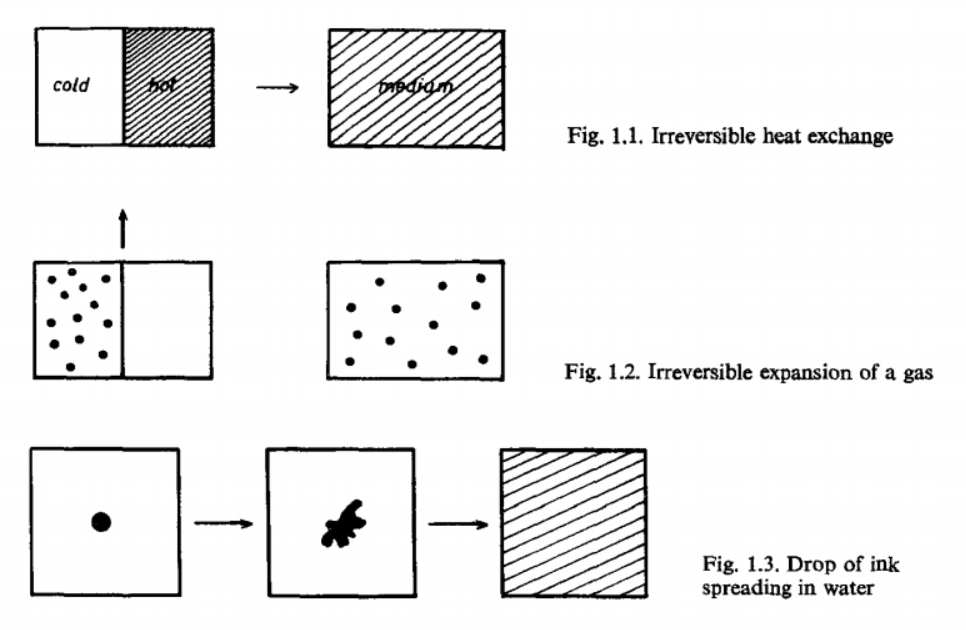
\includegraphics[width=0.8\textwidth]{fig/fig1.1-1.3.png}
        \caption{Irreversible processes: (a) heat exchange, (b) expansion of a gas, (c) Drop of ink
        spreading in water}
    \end{figure}
\end{frame}

\begin{frame}
    In all these cases the systems develop to a unique final state, called a state of \textbf{thermal equilibrium}.
    
    \begin{figure}
        \centering
        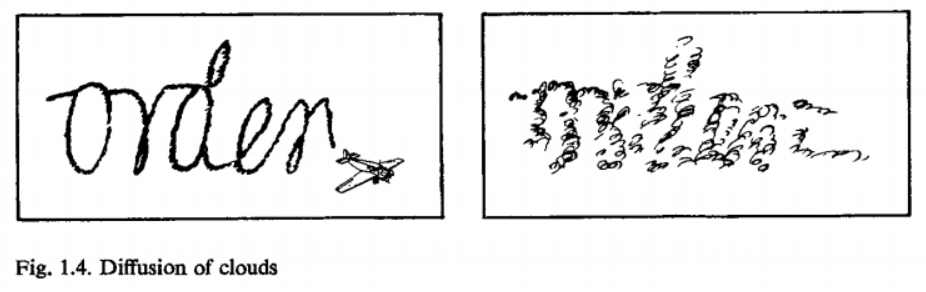
\includegraphics[width=0.8\textwidth]{fig/fig1.4.png}
        \caption{Diffusion of clouds}
    \end{figure}

    \textbf{Disorder is increased}.

\end{frame}

\begin{frame}
    \begin{itemize}
        \item In the realm of thermodynamics, there exists a quantity called \textbf{entropy} which is a measure for the degree of disorder. 
        \item The (phenomenologically derived) laws of thermodynamics state that in a closed system(i.e., a system with no contacts to the outer world) the entropy ever increases to its maximal value.
    \end{itemize}

    \begin{figure}
        \centering
        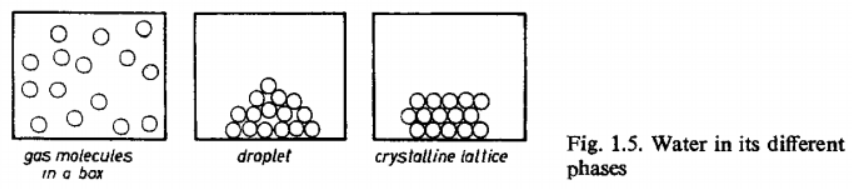
\includegraphics[width=0.8\textwidth]{fig/fig1.5.png}
        \caption{Water in its different phases}
    \end{figure}

    The transitions between the different aggregate states, also called phases, are quite abru
\end{frame}



% -----------------------------------------------------------------------------
\end{document}